\documentclass[a4paper,12pt]{report}

% ================== PAQUETES ==================
\usepackage[utf8]{inputenc}
\usepackage[spanish]{babel}
\usepackage{graphicx}
\usepackage{float}
\usepackage[hidelinks]{hyperref}
\usepackage{caption}
\usepackage{subcaption}
\usepackage{geometry}
\usepackage{titlesec}


% ================== CONFIGURACIÓN DE PAQUETES ==================
\geometry{top=2cm, bottom=2cm, left=2cm, right=2cm}

% ================== INFORMACIÓN DEL DOCUMENTO ==================
\title{Documentación de AppChat}
\author{Zapata Mira, Alberto \\ Cañada Rubio, Laura}
\date{\today}

% ================== INICIO ==================
\begin{document}

% -------- PORTADA --------
\begin{titlepage}
    \begin{center}
    
    % Upper part of the page. The '~' is needed because only works if a paragraph has started.
    
\includegraphics[width=\textwidth]{images/LogosimboloUMU-positivo.png}\\[1cm]
    
    \textsc{\Large }\\[0.5cm]
    
    % Title
    \rule{\linewidth}{0.5mm} \\[0.4cm]
    
    {\huge \bfseries AppChat\\[0.2cm]
    TECNOLOGÍAS DE DESARROLLO DE SOFTWARE \\[0.4cm] }
    
    \rule{\linewidth}{0.5mm} \\[1.5cm]
    
    % Author and supervisor
    \begin{minipage}{0.4\textwidth}
    \begin{flushleft} \large
    \emph{Autor:}\\
    \textsc{Alberto Zapata Mira}\\
    \end{flushleft}
    \end{minipage}
    
    \vfill
    
    % Bottom of the page
    {\large \today}
    
    \end{center}
    \end{titlepage}

% Página en blanco
\newpage
\thispagestyle{empty}
~

% Tabla de contenidos
\newpage
\tableofcontents
\thispagestyle{empty}
\setcounter{page}{0}

% ============= CONTENIDO DEL DOCUMENTO =============
\newpage
\setcounter{page}{1}

\phantomsection
\section*{Historias de Usuario}
\addcontentsline{toc}{section}{Historias de Usuario}

\phantomsection
\subsection*{HU1: Registro de nuevo usuario}
\addcontentsline{toc}{subsection}{HU1: Registro de nuevo usuario}
\begin{description}
  \item[Como:] usuario nuevo
  \item[quiero:] poder registrarme con mi número  de telefono y una contraseña
  \item[para:] poder acceder a la aplicación de mensajería
\end{description}

\textbf{Criterios de aceptación:}
\begin{itemize}
    \item El usuario puede introducir un número valido y una contraseña segura.
    \item El sistema valida el número y muestra errores claros si es incorrecto.
    \item El sistema informa si el número ya está registrado.
\end{itemize}

\phantomsection
\subsection*{HU2: Inicio de sesión}
\addcontentsline{toc}{subsection}{HU2: Inicio de sesión}
\begin{description}
  \item[Como:] usuario registrado
  \item[quiero:] iniciar sesión con mis credenciales
  \item[para:] acceder a mis contactos y conversaciones
\end{description}

\textbf{Criterios de aceptación:}
\begin{itemize}
    \item El usuario puede ingresar su número y contraseña correctamente.
    \item Si las credenciales son inválidas, el sistema muestra un mensaje de error.
    \item El acceso es denegado hasta que las credenciales sean válidas.
\end{itemize}

\phantomsection
\subsection*{HU3: Añadir contacto}
\addcontentsline{toc}{subsection}{HU3: Añadir contacto}
\begin{description}
  \item[Como:] usuario
  \item[quiero:] poder añadir nuevos contactos mediante su identificador
  \item[para:] poder comunicarme con ellos desde la aplicación
\end{description}

\textbf{Criterios de aceptación:}
\begin{itemize}
    \item El sistema permite buscar usuarios por identificador.
    \item Se muestra un mensaje si el usuario no existe.
    \item El contacto se añade a la lista del usuario tras la confirmación.
\end{itemize}

\phantomsection
\subsection*{HU4: Crear grupo}
\addcontentsline{toc}{subsection}{HU4: Crear grupo}
\begin{description}
  \item[Como:] usuario
  \item[quiero:] poder crear grupos de conversación
  \item[para:] mantener conversaciones con múltiples contactos al mismo tiempo
\end{description}

\textbf{Criterios de aceptación:}
\begin{itemize}
    \item El usuario puede nombrar el grupo y seleccionar contactos.
    \item El grupo se guarda con la información y miembros indicados.
    \item Se puede ver el grupo creado en la lista de grupos.
\end{itemize}

\phantomsection
\subsection*{HU5: Enviar mensaje}
\addcontentsline{toc}{subsection}{HU5: Enviar mensaje}
\begin{description}
  \item[Como:] usuario
  \item[quiero:] poder enviar mensajes de texto a mis contactos o grupos
  \item[para:] comunicarme con mis contactos.
\end{description}

\textbf{Criterios de aceptación:}
\begin{itemize}
    \item El usuario puede escribir y enviar mensajes.
    \item Los mensajes se muestran inmediatamente en el chat.
    \item Los destinatarios reciben el mensaje cuando se conectan.
\end{itemize}

\phantomsection
\subsection*{HU6: Ver historial de conversaciones}
\addcontentsline{toc}{subsection}{HU6: Ver historial de conversaciones}
\begin{description}
  \item[Como:] usuario
  \item[quiero:] poder ver el historial de mensajes de mis conversaciones
  \item[para:] seguir el contexto de la conversación
\end{description}

\textbf{Criterios de aceptación:}
\begin{itemize}
    \item El historial de cada chat se carga al abrirlo.
    \item El usuario puede desplazarse y leer mensajes anteriores.
    \item Los mensajes aparecen en orden cronológico.
\end{itemize}

\phantomsection
\subsection*{HU7: Gestionar Contactos y Grupos}
\addcontentsline{toc}{subsection}{HU7: Gestionar Contactos y Grupos}
\begin{description}
  \item[Como:] usuario
  \item[quiero:] poder gestionar mis contactos y grupos
  \item[para:] mantener mi lista de contactos y grupos actualizada
\end{description}

\textbf{Criterios de aceptación:}
\begin{itemize}
    \item El usuario puede acceder a un formulario de edición.
    \item Los cambios se guardan y se reflejan inmediatamente.
    \item El sistema valida los campos antes de guardar.
\end{itemize}

\phantomsection
\subsection*{HU8: Cerrar sesión}
\addcontentsline{toc}{subsection}{HU8: Cerrar sesión}
\begin{description}
  \item[Como:] usuario
  \item[quiero:] poder cerrar sesión de forma segura
  \item[para:] proteger el acceso a mi cuenta
\end{description}

\textbf{Criterios de aceptación:}
\begin{itemize}
    \item Hay una opción accesible para cerrar sesión.
    \item Al cerrar sesión se redirige al usuario a la pantalla de inicio.
    \item No se puede acceder a funciones privadas tras cerrar sesión.
\end{itemize}

\newpage
\phantomsection
\section*{Diagrama de Clases UML}
\addcontentsline{toc}{section}{Diagrama de Clases UML}

\begin{figure}[H]
    \centering
    \begin{minipage}{0.85\textwidth}
        \centering
        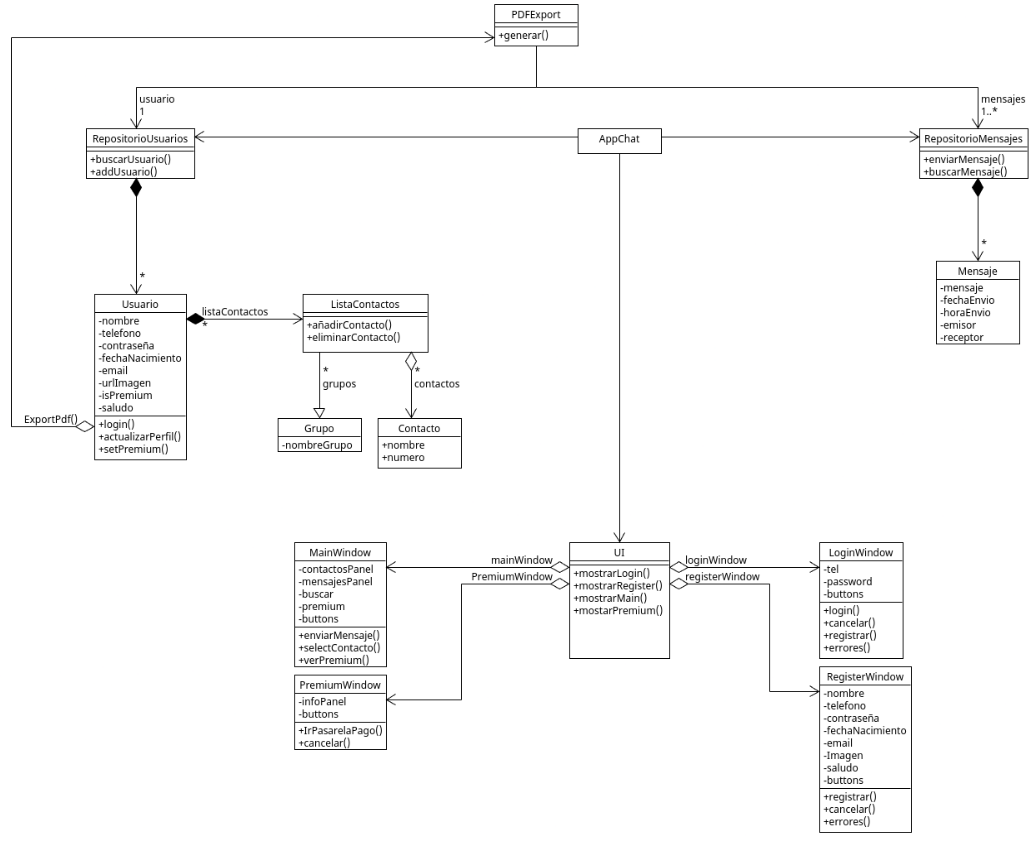
\includegraphics[width=\textwidth]{images/AppChat_Dominio_Inicial.png}
        \caption*{Diagrama de clases - versión inicial}
    \end{minipage}
    
    \vspace{1.5em}

    \begin{minipage}{0.85\textwidth}
        \centering
        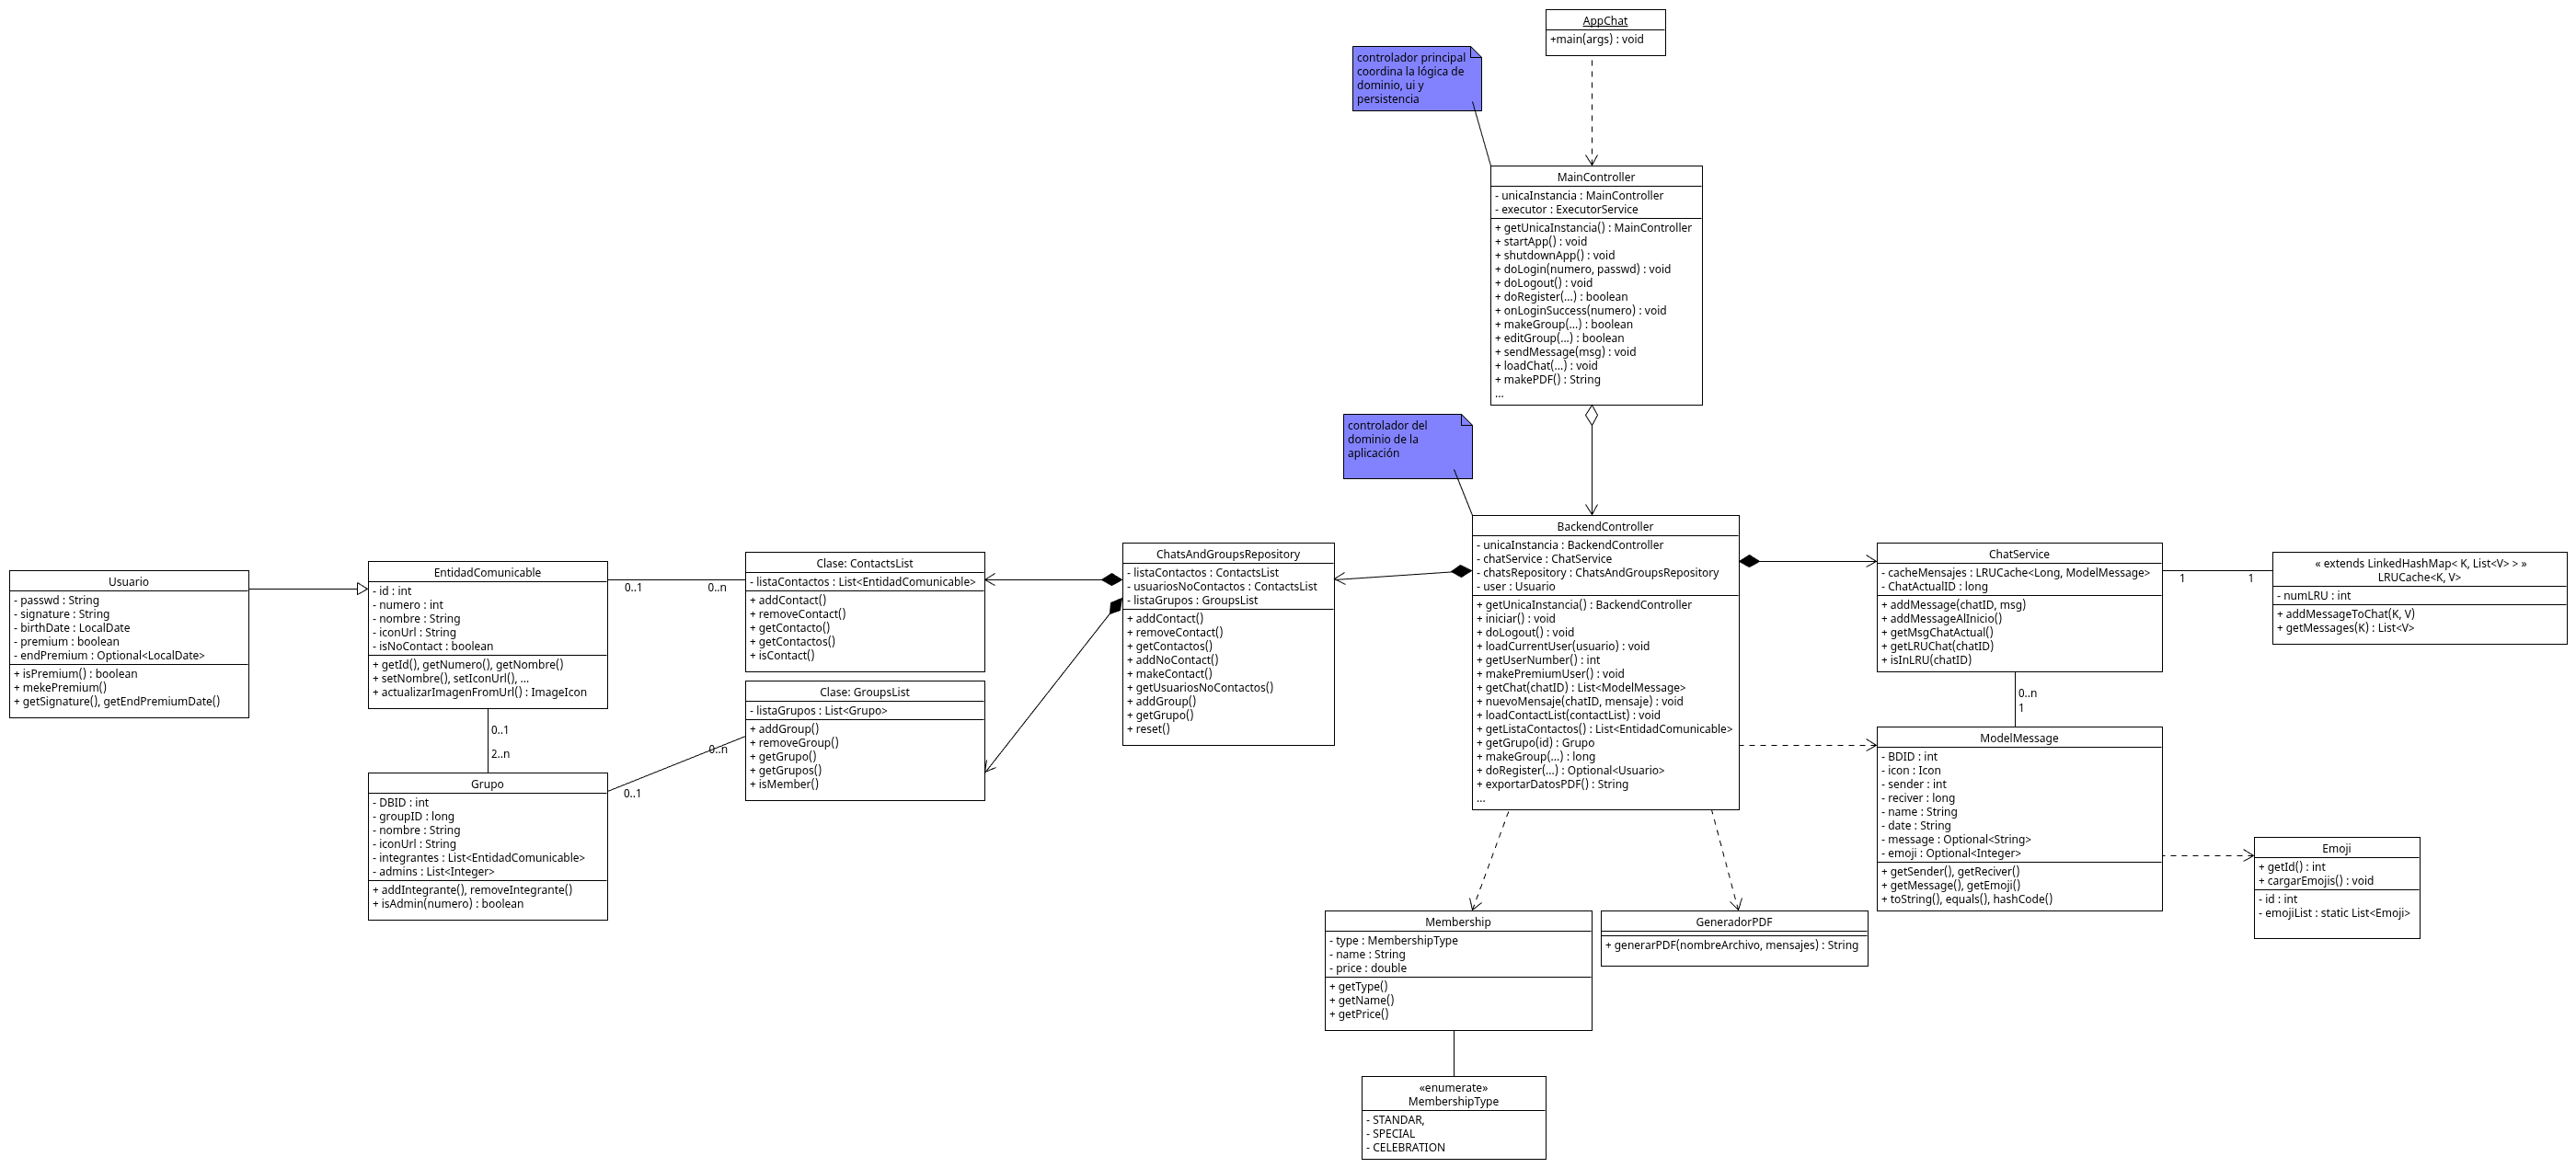
\includegraphics[width=\textwidth]{images/AppChat_Dominio.png}
        \caption*{Diagrama de clases - versión final}
    \end{minipage}
\end{figure}

\phantomsection
\section*{Diagrama de Secuencia: Añadir Contacto a Grupo}
\addcontentsline{toc}{section}{Diagrama de Secuencia: Añadir Contacto a Grupo}

\begin{figure}[H]
    \centering
    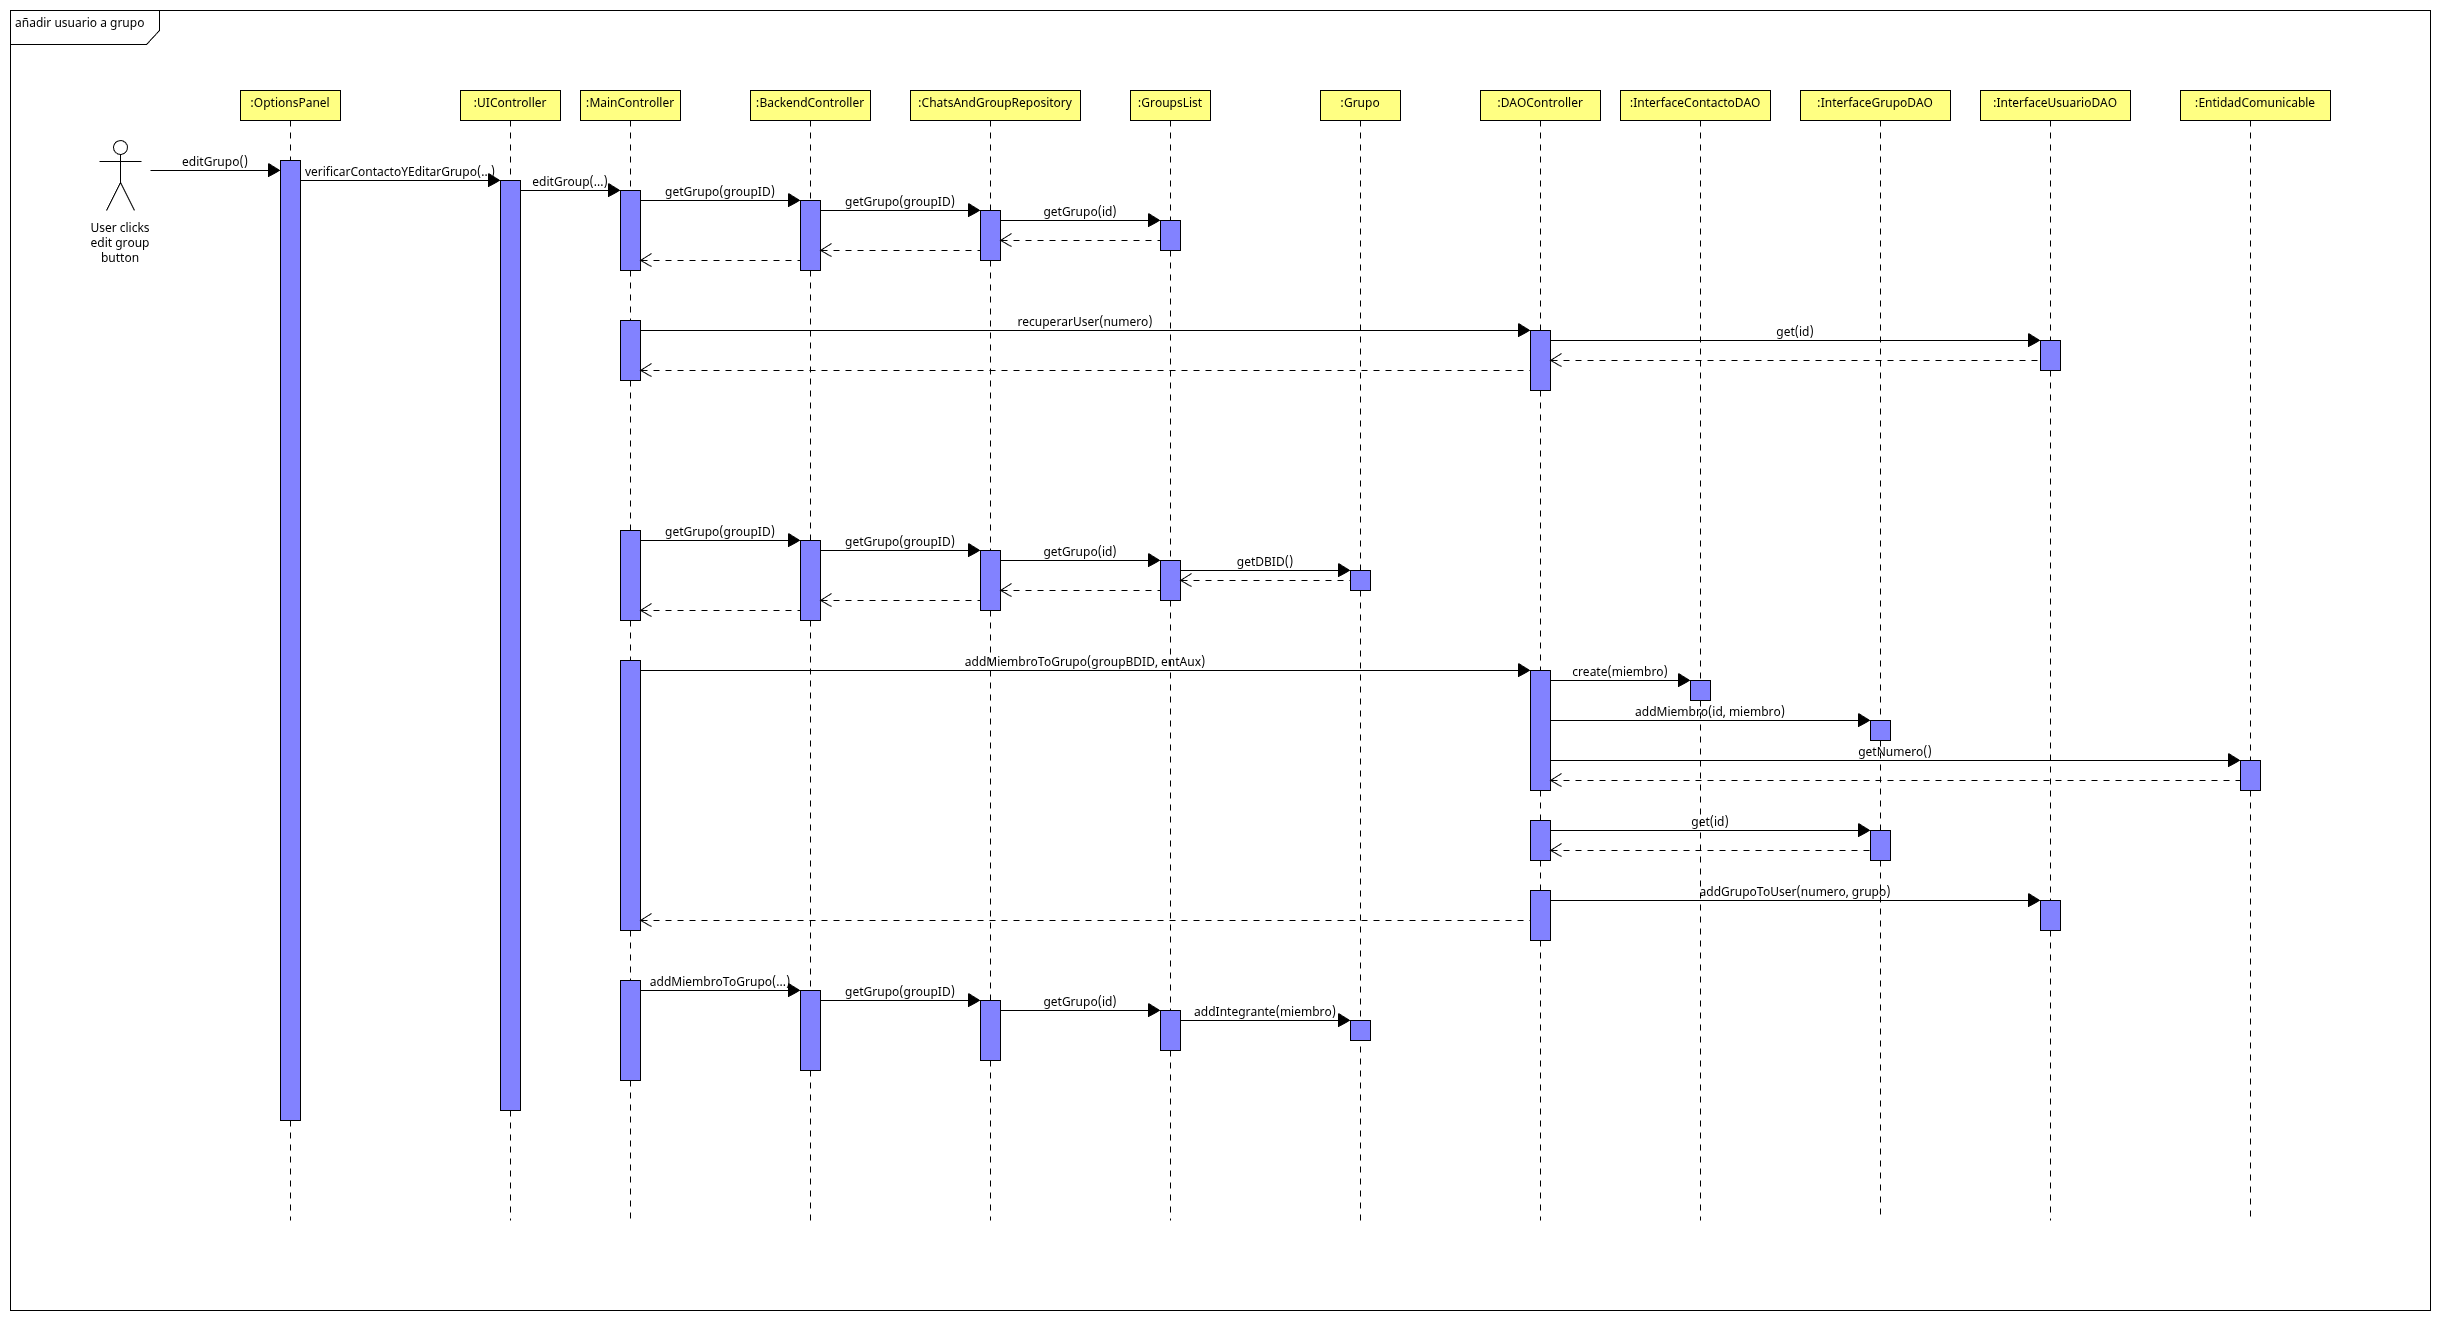
\includegraphics[width=0.9\textwidth]{images/addUserToGroupSequence.png}
    \caption{Secuencia para añadir un contacto a un grupo}
\end{figure}

\chapter{Arquitectura de la Aplicación}

Breve explicación de la arquitectura utilizada. Por ejemplo: patrón MVC, capas de presentación, lógica y datos, etc.

Decisiones de diseño importantes tomadas durante el desarrollo.

\section*{Patrones de Diseño}
\addcontentsline{toc}{section}{Patrones de Diseño}

Se describen los patrones utilizados, ya sea explícitamente o mediante librerías como Swing, DAO, etc.

\section*{Manual de Usuario}
\addcontentsline{toc}{section}{Manual de Usuario}

Instrucciones básicas para utilizar la aplicación:
\begin{itemize}
    \item Cómo iniciar sesión
    \item Cómo añadir un contacto
    \item Cómo crear un grupo
    \item ...
\end{itemize}

\section*{Observaciones Finales}
\addcontentsline{toc}{section}{Observaciones Finales}

Tras realizar el proyecto, lo cual me ha transmitido una sensación de satisfacción, puesto que ha sido el
proyecto más completo que he realizado hasta el momento, he sacado las siguientes conclusiones:
\begin{itemize}
    \item La importancia de la planificación, especialmente en la persistencia y la interfaz de usuario, pues fáclita mucho el desarrollo.
    \item La necesidad de realizar pruebas para garantizar el funcionamiento de la aplicación tras realizar cambios.
    \item La utilidad de los patrones de diseño en la arquitectura del software. Pues estos suelen ser la respuesta a una necesidad surgida durante el desarrollo.
    \item La utilidad de refactorizar el código, tanto como sea posible en el margen de tiempo disponible,  pues el aprendizaje es continuo y el código se puede mejorar en casi todas las ocasiones.
\end{itemize}

El proyecto dispone de un repositorio de GitHub donde se puede obtener información referente a la ejeución, requisitos y betas de la aplicación: 
\textcolor{blue}{\href{https://github.com/StoneySpring688/AppChat_2024-2025}{Repositorio}}


\subsection*{Estimación de tiempo dedicado}

Estimo entre 50 y 60 horas de trabajo.


\end{document}
